\subsubsection{Analyse de l'overfitting}

Afin de vérifier la capacité de généralisation du modèle retenu, une courbe
d'apprentissage a été générée pour la \textbf{Régression Logistique}. Cette
courbe compare le ROC-AUC obtenu sur l'ensemble d'entraînement et sur
l'ensemble de validation pour différentes tailles d'échantillons.

\begin{figure}[H]
\centering
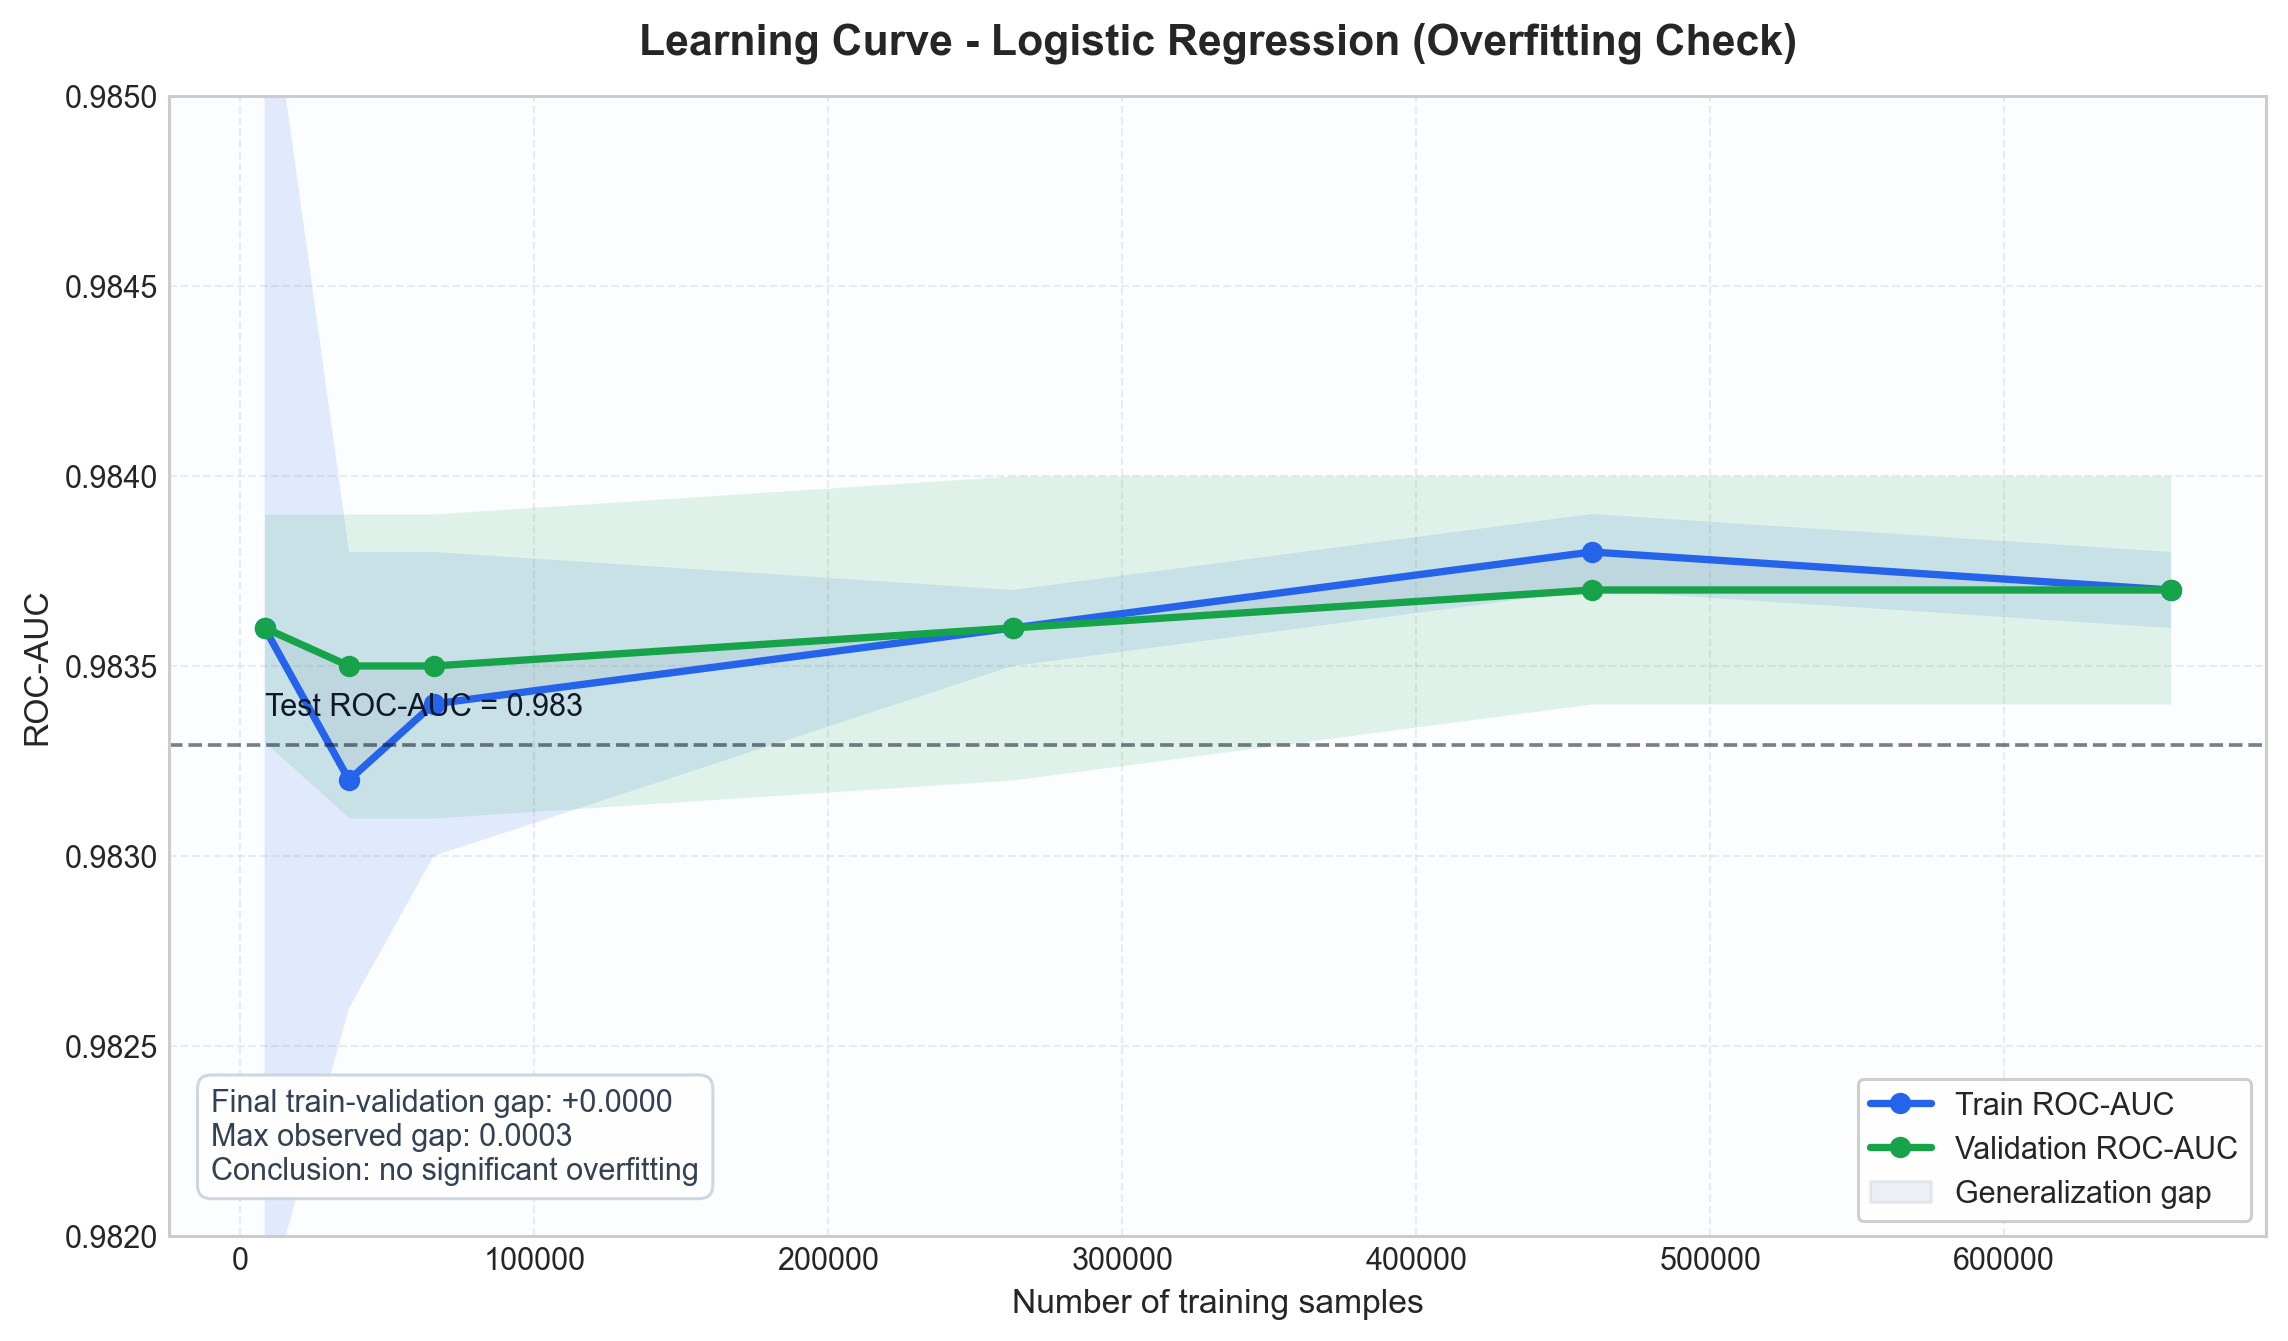
\includegraphics[width=0.95\textwidth]{reports/churn_model_comparison/churn_logistic_overfitting_curve_roc_auc.png}
\caption{Courbe d'apprentissage de la Régression Logistique pour le contrôle de l'overfitting}
\label{fig:churn-logistic-overfitting}
\end{figure}

\medskip

Les deux courbes restent très proches lorsque le nombre d'échantillons
d'entraînement augmente. Le ROC-AUC final est d'environ \textbf{0,983} sur
l'ensemble de test, tandis que l'écart maximal observé entre l'entraînement et
la validation reste très faible, autour de \textbf{0,0003}.

\medskip

Cette stabilité indique que le modèle ne mémorise pas excessivement les données
d'entraînement. La \textbf{Régression Logistique} présente donc une bonne
capacité de généralisation, ce qui renforce son choix comme modèle final pour
la prédiction du churn. Elle combine ainsi une performance élevée, une faible
tendance à l'overfitting et une forte interprétabilité métier.
